\hspace*{0.6cm}Судалгааны үйл явцыг илүү сайн ойлгохын тулд 5 үе шатанд хуваасан. Үе шат бүрд дараагийн шатанд бэлтгэх, хэрэгжүүлэлтийн талаар туршлага хуримтлуулах, үүссэн өгөгдлийг хэмжиж, цуглуулах тодорхой үйлдлүүдийг гүйцэтгэнэ. Зураг \ref{fig:phases}-д судалгааны үйл явцын үе шатууд болон тэдгээрийг хэрэгжүүлэх дарааллыг харуулав.
\subsubsection{Сэдвийн судлагдсан байдал, хүрээг тодорхойлох}
\hspace*{0.6cm}Энэ үе шатны зорилго нь сэдвийн ойлголттой танилцахад оршино. Шаардлагатай мэдлэг- ийн түвшинд хүрэхийн тулд Scopus, DiVA (Дэд бүлэг \ref{sec:literature-review}-ыг үзнэ үү) өгөгдлийн сангаас гадна төрөл бүрийн блог, форум, фрэймворкүүдийн техникийн баримт бичгүүдийг ашигласан. Энд ISO/IEC 25010 стандартыг судалж, МУИС-ийн Дипломын ажлын удирдлагын системд шаардлага- тай байж болох программ хангамжийн чанарын үзүүлэлтүүдийн тодорхойлолтыг гаргасан.
\subsubsection{Туршилтын загвар}
\hspace*{0.6cm}Фронтэнд хөгжүүлэлтэд микрофронтэнд архитектурыг хэрэгжүүлэх техникийн мэдлэг, туршлага хуримтлуулах зорилгоор туршилтын загварыг (Дэд бүлэг \ref{sec:prototype}-ыг үзнэ үү) хөгжүүлсэн. Туршлага хуримтлуулахаас гадна, хэрэгжүүлэлтийн явцад төрөл бүрийн сорилт, бэрхшээлүүд гарч ирсэн болно. Туршилтын загвар нь React,JSF гэсэн хоёр өөр фрэймворкоор хөгжүүлэгдсэн, микрофронтэнд аппликэйшнүүдийг ачаалдаг жижиг хэмжээний аппликэйшн юм.

\subsubsection{Туршилт}
\hspace*{0.6cm}Туршилтын үе шат (Дэд бүлэг \ref{sec:experiment}-ийг үзнэ үү) нь МУИС-ийн Дипломын ажлын удирдлагын системийн хэрэглэгчийн интерфейсийг цэвэр микрофронтэнд болон холимог микрофронтэнд архитек- тураар хөгжүүлэх үйл явцаас бүрдэнэ. Хөгжүүлэлтийн давтамж бүрийн дараа санал болгож буй шийдлийг сонгогдсон ISO/IEC 25010 чанарын үзүүлэлтүүд болон микрофронтэнд архитектурын үндсэн зарчмуудтай уялдуулан үнэлэв.

\subsubsection{Кэйс судалгаа}
\hspace*{0.6cm}Кэйс судалгааны объект нь МУИС-ийн Дипломын ажлын удирдлагын систем бөгөөд харьцуулах хоёр хувилбарыг тодорхойлов: нэгдүгээрт, JSF~2.2 монолит архитектур; хоёрдугаарт, Vite Module Federation ашиглан хэрэгжүүлсэн React MFE болон Spring WebFlux реактив микросервис архитектур. Судалгааны нэгж нь нэг системийн хоёр архитектурын хувилбарыг ижил функциональ шаардлага, ижил туршилтын орчинд (Apple M2 Pro, macOS~15.3, localhost) хэмжсэн нэг кэйс зохиомж юм. Хэмжигдэх үзүүлэлтүүдийг дөрвөн бүлэгт хуваав: хөгжүүлэлтийн хурд (Lead Time, HMR/reload), ажлын ачааллын гүйцэтгэл (RAM, латенц), сүлжээний зардал (payload, кэш), кодын чанар (Cyclomatic Complexity, duplication).

\subsubsection{Өгөгдлийн шинжилгээ}
\hspace*{0.6cm}Цуглуулсан өгөгдлийг хоёр аргачлалаар шинжиллэв. Нэгдүгээрт, ISO/IEC~25010 стандартын 7 чанарын үзүүлэлт (Хугацааны төлөв, Харилцан ажиллах чадвар, Модульлаг байдал, Дахин ашиглах боломж, Шинжилж болохуйц байдал, Өөрчлөх боломж, Тестлэх боломж)-ийг Google Lighthouse, SonarQube, madge, Jest, Cypress хэрэгслүүдийн тоон гаралтаар хэмжиж, JSF болон React MFE архитектурыг харьцуулан оноолов. Хоёрдугаарт, ATAM (Architecture Trade-off Analysis Method) аргачлалаар архитектурын гол шийдвэрүүдийн мэдрэмтгий цэг (Sensitivity Point) болон буулт цэгүүдийг (Trade-off Point) тодорхойлж, чанарын үзүүлэлтүүдийн хоорондох өрсөлдөөнт харилцааг шинжиллэв.

\begin{figure}[h!]
	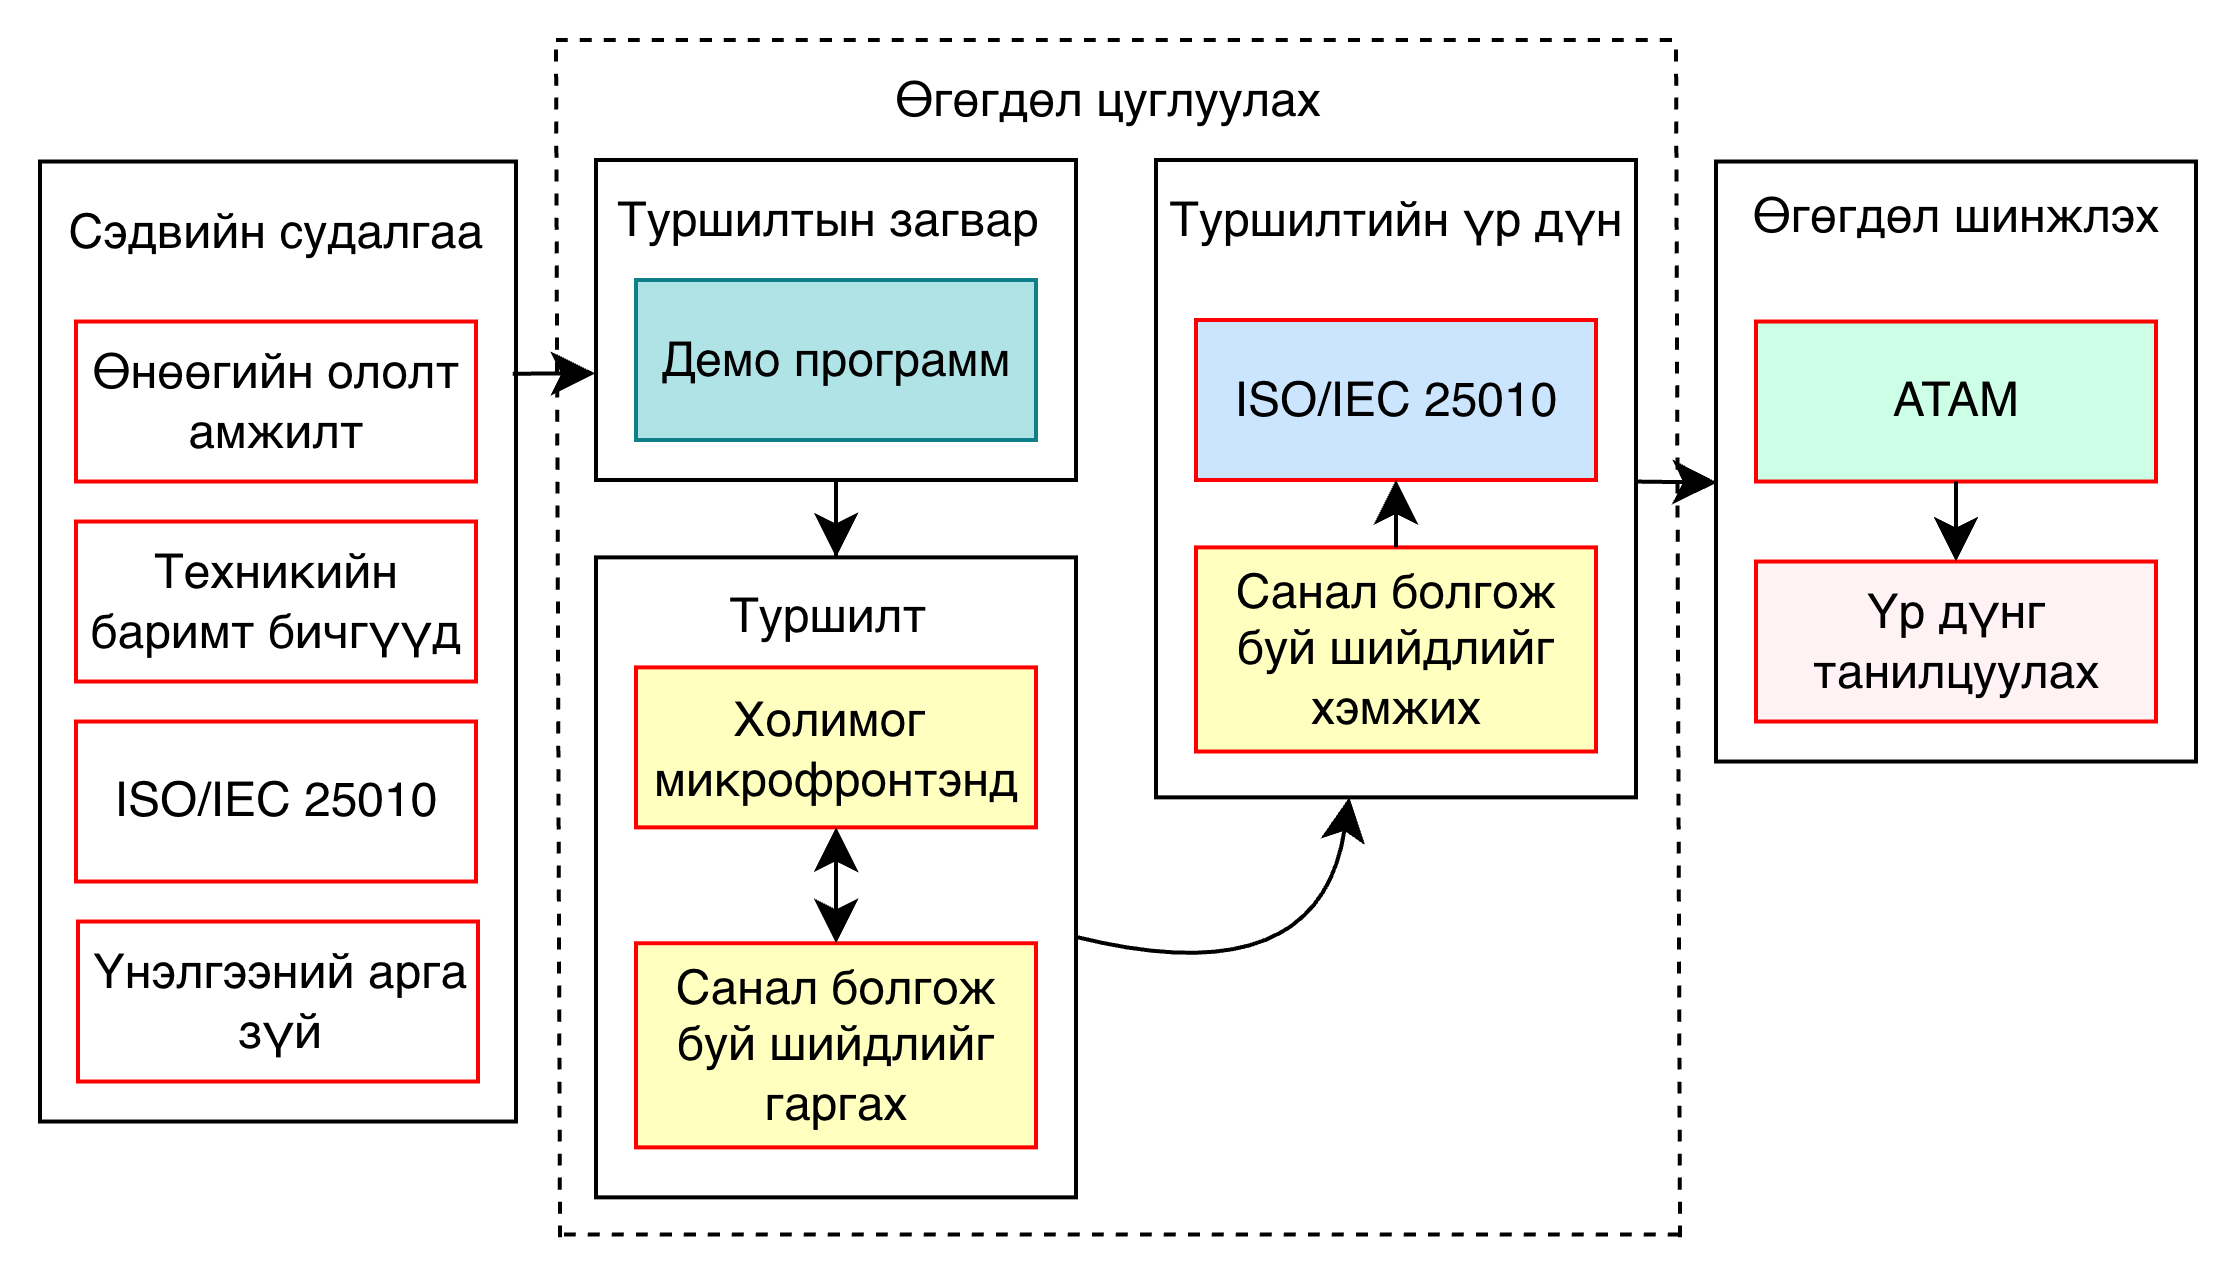
\includegraphics[width=17cm]{images/phases.png}
	\caption{Судалгааны үйл явцын үе шатууд}
	\label{fig:phases}
\end{figure}